% git_best_practices.tex
\documentclass{beamer}
\usetheme[hideothersubsections,height=6mm]{Berkeley}
\usefonttheme{structuresmallcapsserif}
\setbeamertemplate{navigation symbols}{}

\usepackage{color}
\usepackage[ascii]{inputenc}
\usepackage{hyperref}


\title{Git Use Cases}
\subtitle{Subtitle? pft...}
\author{Jake Tobak}
\institute{Engineering and Computer Science Interest Group \\
           URI Student ACM Chapter}
\date{6 March 2013}
\logo{
\includegraphics[height=1cm]{logo_simple.png}}

\begin{document}

\frame{\titlepage}

\begin{frame}{Outline}
  \tableofcontents
\end{frame}


\section{Single Developer Project}
\begin{frame}{Backup Code}
  \begin{itemize}
  \item The Wrong Way\\
          Keep your source on Dropbox
  \pause
  \item Why?\\
        For a single developer project, dropbox isn't a terrible alternative to Git for keeping a backup of your current source code, but Git is more than a server to keep a backup of your latest version of code.
  \pause
  \item The Git Way\\
        Use Git!
  \pause
  \item Why?\\
        Cause Git!
  
  \end{itemize}
  

\end{frame}

\begin{frame}{Restore Previous Version}
  You want to revert to a previous version of your code, back when everything actually worked.
  \begin{itemize}
  \item The Wrong Way\\
          Keep your source on Dropbox
  \pause
  \item Why?\\
        Dropbox does allow you to restore previous versions of your files for up to 30 days, or even longer if you subscribe to their Packrat service, but it's only available to Pro users (starting at \$10/month) and costs \$40/year on top of that. It also doesn't give you a summary of the changes between each version other than the date and user who made them.
        \end{itemize}
\end{frame}

\begin{frame}{Restore Previous Version (cont.)}
\begin{itemize}
  \item The Wronger Way\\
          Keep multiple versions of your code saved locally
  \pause
  \item Why?\\
        This can get real messy and real confusing real quick. There's also no explanation of what was changed in each version or a clear chain of progression.
  \pause
  \item The Wrongest Way\\
          Reopen the source in your editor and hold CTRL+Z until the buffer runs out.
  \pause
  \item Why?\\
        How far back does your undo buffer go? Will it go back to a working state or stop short? How do you know when you got to that spot where everything is working and not a couple places before/after you changed that = to a ==?
        \end{itemize}
\end{frame}

\begin{frame}{Restore Previous Version (cont.)}
\begin{itemize}
  \item The Git Way\\
        \textbf{git commit} and \textbf{git push} every time you make a significant change. Then \textbf{git log} and \textbf{git checkout} to revert to a previous version.
  \pause
  \item Why?\\
        \textbf{git commit} stages all the changes you made to your code since the last update and lets you give a brief explanation of what has changed since then. \textbf{git push} uploads the staged changes to your git server.\\
        \textbf{git log} allows you to view your previous commits with an explanation of what you did in each one. You can use \textbf{git checkout} to download a copy of a specific version to your computer.
  \end{itemize}
  

\end{frame}





\section{Multi Developer Project}
\begin{frame}{Working on different files}
\begin{itemize}
\item The Wrong Way\\
        Everyone on the team e-mails each other their latest source files and tells everyone what they'll be working on.
  \pause
  \item Why?\\
        This will take forever if you have to wait for someone to e-mail you a piece of code you need and it's very easy to have branches that are extremely divergent to each other.
  
  \pause
  \item The Also Wrong Way\\
        Share a Dropbox account
  \pause
  \item Why?\\
        This will work, but if you're both working at the same time and another developer saves a change to test it, you might sync a broken file and start getting errors for something someone else did. Have fun debugging that.
  \end{itemize}

\end{frame}


\begin{frame}{Working on different files (cont.)}
\begin{itemize}
\item The Git Way\\
        Just do it!\\
\pause
        When you \textbf{push} to the git server, you're uploading your changes, but you can also \textbf{pull} the changes from the server that have been made since the last time you sync'd with it.
  \pause
  \item Why?\\
        If you're working on the same \textbf{branch}, git will \textbf{merge} your changes and any changes other people have made since your last \textbf{push/pull}. Git will attempt to automatically combine everyone's changes in a way that won't break anything. Git is really clever.
\end{itemize}
\end{frame}

\begin{frame}{Working on the SAME files}
\begin{itemize}
\item The Wrong Way\\
        I don't even know, just don't.
\pause
\item The Git Way\\
        Do it, you won't do it!
\pause
  \item Why?\\
        Seriously, Git is REALLY clever when it comes to merging. I'm sure you could break it if you wanted to, but if you don't \textbf{push} broken code or really redonkulous changes, everything will probably be fine.
\end{itemize}
\end{frame}

\begin{frame}{Making Radical Changes}
  \begin{itemize}
    \item The Wrong Way\\
            I would hope that you would know better than to not use Git by now, but there are wrong ways to use Git too.\\
            Just continue with business as usual using Git.
    \pause
    \item Why?\\
            If you're adding a new feature or something big, you might need to \textbf{commit} and \textbf{push} multiple times before your code is working perfectly again. If anyone does a \textbf{pull} before you're done, they'll have incomplete code merged into their source and it'll cause a lot of headaches. It's also possible that you only \textbf{push} working code, but maybe someone had a better solution that your team will go with instead and you'll just be competing against each other every time you \textbf{push}.
          \end{itemize}
          \end{frame}
\begin{frame}{Making Radical Changes}
  \begin{itemize}
    \item The Git Way\\
            \textbf{branch}! You can use \textbf{git branch} to create a new \textbf{branch}. A \textbf{branch} is a chain of \textbf{commits} that diverges from the current history. When you \textbf{push} to a new \textbf{branch}, it won't be merged when someone \textbf{pulls} from the original. When you're satisfied with your code, you can \textbf{pull} your code from the new \textbf{branch} into the original and Git will attempt to \textbf{merge} everything for you.
  \end{itemize}
\end{frame}

\section{Open Source Project}

\begin{frame}{Contributing to Open Source}
  Open Source Projects are Multi Developer Projects, but you don't have write access! How can you contribute while having read-only permission?\\
    \pause
  The solution is \textbf{git clone}. When you \textbf{clone}, you are creating a copy of the \textbf{repository} (repo) that includes all the code, history and branches, but this copy belongs to you and you can do whatever you want with it. \textbf{commits} you make will be completely independent of the original source. \textbf{forking} is GitHub's version of \textbf{clone}, but it creates the repo under your GitHub account.
\end{frame}

\begin{frame}{Contributing to Open Source (cont.)}
  Okay, so now you can edit the code, but you're still doing it in your own \textbf{repo}. The original project is unaware of your changes, so what good are ya?\\
  
  \pause
  The solution is \textbf{git request-pull}. \textbf{request-pull} generates a summary of the changes you made and a URL to find them. You can then post this to a mailing list or send it to the person incharge of the original project. If they like what they see, they can \textbf{pull} from your code and \textbf{merge} it into the original project. You can also generate a \textbf{patch} that is a list of the changes between your version and the original version, which they might prefer.
  \end{frame}
  \begin{frame}{Contributing to Open Source (cont.)}
  Another solution is GitHub's \textbf{Pull Request}. It's similar to the native \textbf{request-pull} and \textbf{patch} process, but it's much more interactive and can be managed from a web interface. If an Open Source Project is hosted on GitHub, then this is probably how they want you submit your changes.
  \vfill
  \pause
  The best way to find out how you can contribute to a project is to join its IRC channel and/or mailing list.
\end{frame}


\section{Workflow}
\begin{frame}{General Workflow}
 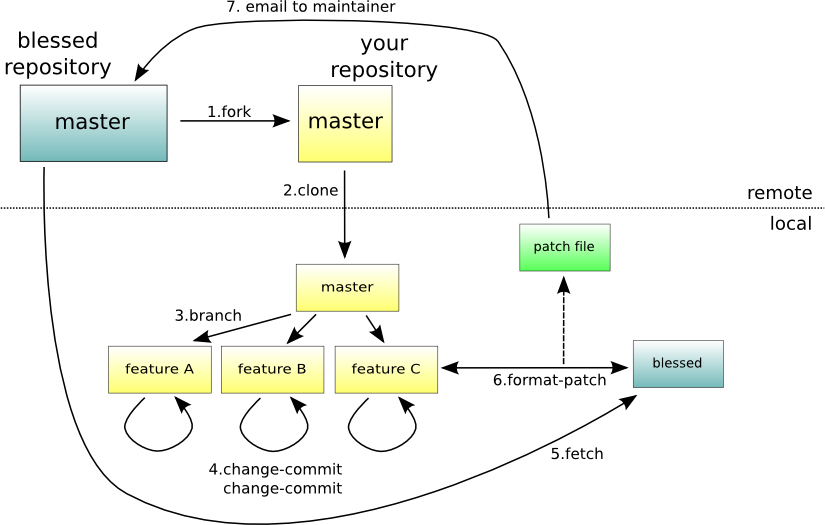
\includegraphics[width=300px]{workflow.png}
\end{frame}


\end{document}
